%第3章2
\section{設計}
\subsection*{基本設計}

ユースケース図の動作を満たすように基本設計を行う。図\ref{class}を基に、基本設計を行った。

図\ref{class}に示されている項目をもとに、機能別にクラス化を行った。クラスには、カゴ、解析システム、カゴDB、決済システム、商品DBがある。
クラス名カゴの役割は、ユーザがカート内に商品を出し入れする動作全般を行う。クラス名解析システムの役割は、カートに入れられた商品の識別を行う。
カゴDBの役割は、カートに入れられた商品の管理を行うためにある。決済システムの役割は、ユーザが決済を行う際の購入金額の計算および、カゴDBの整理を行う。最後の商品DBの役割は、商品の値段や、商品名、バーコード番号の管理を行うためにある。

図\ref{class}はカゴ、解析システム、カゴDB、商品DB、決算システム、それぞれの操作を示したクラス図である。カゴクラスでは、ユーザが商品を出し入れする際に、その商品の画像データを確保する。また、ユーザに解析が成功したかの通知を行う。解析システムクラスでは、カゴから送られてきたデータの受信、解析とカゴDBへの操作を行う。カゴDBでは、ユーザが購入予定の商品の管理を行う。商品DBでは、商品のバーコード番号と商品名、値などの商品情報を管理している。店側が新しい商品を追加する場合は、このDBに商品情報を追加する必要がある。最後の決済システムでは、ユーザが決済する際に必要な処理を行う。

次に、クラスごとの動作要件を満たす検証項目を表\ref{join_test}に示す。

\begin{figure}[htbp]
\centering
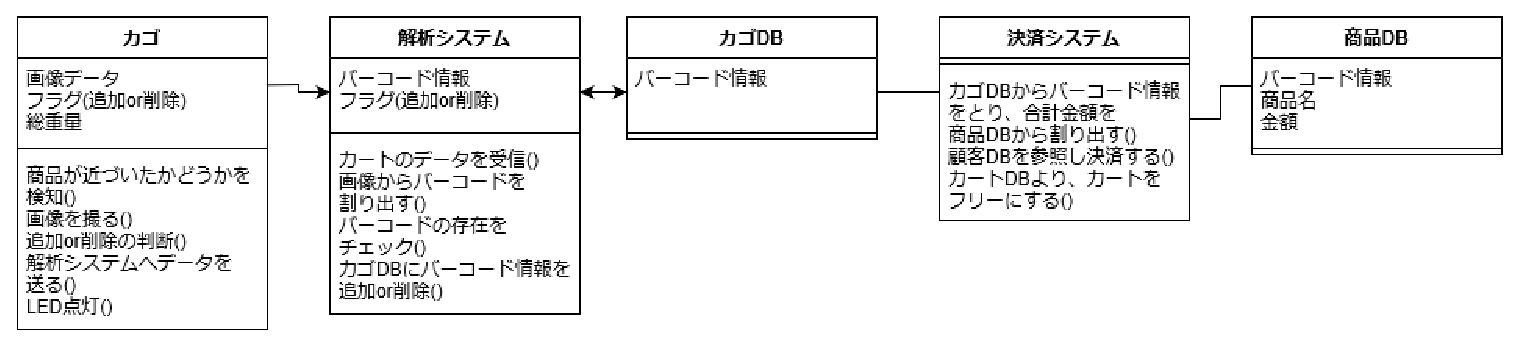
\includegraphics[width=15cm]{./pic/class_final.eps}
\caption{クラス図}
\label{class}
\end{figure}

\begin{table}[htbp]
\centering
\label{join_test}
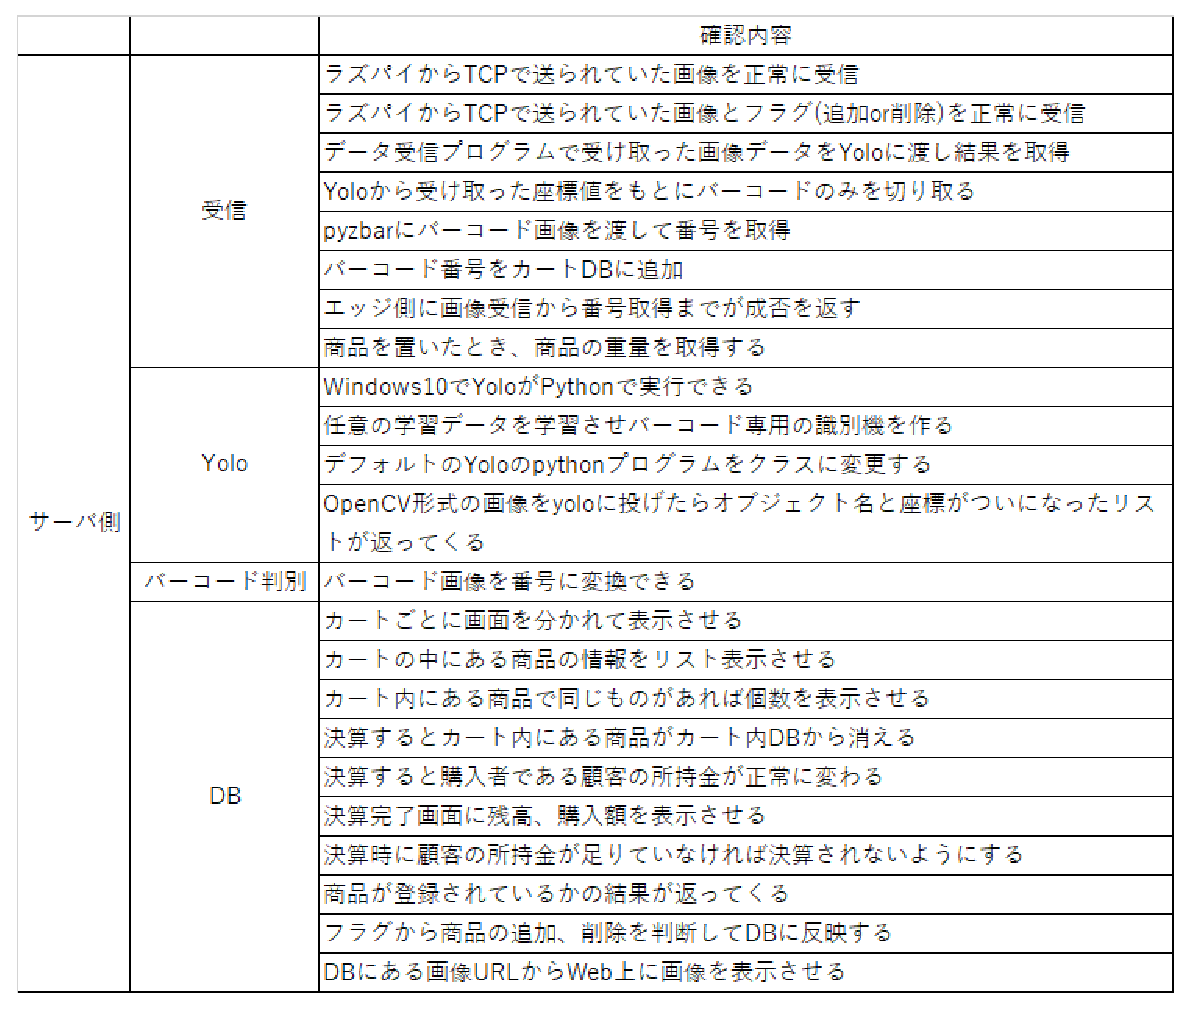
\includegraphics[width=15cm]{./pic/join_test.eps}
\caption{結合テスト項目}
\end{table}